\documentclass{article}
\usepackage[utf8]{inputenc}
\usepackage{algorithm}
\usepackage{algpseudocode}
\usepackage{amsmath}
\usepackage{amsthm}
\usepackage{amsfonts}
\usepackage{graphicx}
\usepackage{geometry}
\geometry{a4paper, portrait, margin=1in}

\theoremstyle{plain}
\newtheorem{thm}{Theorem}

\theoremstyle{definition}
\newtheorem{defn}{Definition} % definition numbers are dependent on theorem numbers
\newtheorem{exmp}{Example} % same for example numbers

\title{Machine Intelligence (UE18CS303) \\
\large Unit 2}
\author{Aronya Baksy}
\date{September 2020}

\begin{document}
    \maketitle
\section{K-Nearest Neighbours Classification}
\subsection{Instance Based Learning}
\begin{itemize}
    \item The K-nearest neighbours algorithm is an \textbf{instance-based} learning algorithm
    
    \item In an instance-based algorithm the training phase consists only of storing the data
    
    \item When a query with some previously unseen data point is made to the algorithm, the most similar instances are used to classify the unseen query instance.
\end{itemize}

\subsection{K-Nearest Neighbours Algorithm}
\begin{itemize}
    \item The KNN algorithm considers each training instance to be represented as a single point in an $n$-dimensional Euclidean space $\mathbb{R}^n$
    
    \item An arbitrary instance $x$ can be represented using the feature vector
    $\langle a_1(x), a_2(x), a_3(x), ..., a_n(x) \rangle$ where $a_r(x)$ denotes the value of the $r^{th}$ attribute of point $x$. 
    
    \item The distance measure used to compute the distance between two examples $x_i$ and $x_j$ is given by the Euclidean Distance Formula
    
    \begin{equation}
        d(x_i, x_j) = \sqrt{\sum_{r=1}^{n} (a_r(x_i) - a_r(x_j))^2}
    \end{equation}
    
    \item The target function to be learnt is denoted as $f(x)$ and it takes a discrete set of values $V$ (which are the classes of the classification algorithm). 
    
    \item Given an unseen query instance $x_q$, the algorithm assigns the \textbf{most common class} from among the \textbf{$k$ closest training examples} to the query instance. 
\end{itemize}

\begin{algorithm}
    \caption{K-Nearest Neighbours}
    \begin{algorithmic}
        \Procedure{KNN\_Train}{$\langle x, f(x) \rangle$}
            \State Add the example $\langle x, f(x) \rangle$ to the list of examples
        \EndProcedure\\
        \Procedure{KNN\_Classify}{$x_q$: Query Instance}
            \State $x_1, x_2, x_3, ..., x_k \gets  $ The $k$ closest train examples to $x_q$
            
            \State $f(x_q) \gets \operatorname*{argmax}\limits_{v \in V}  \sum\limits_{i=1}^{k} \delta(v, f(x_i))$
            
            \Return $f(x_ q)$
        \EndProcedure
    \end{algorithmic}
\end{algorithm}

\begin{itemize}
    \item Here, $\delta(a, b) = 1$ if $a==b$ else $\delta(a, b) = 0$
\end{itemize}
\subsection{Distance Weighted K-nearest Neighbours }

\begin{itemize}
    \item The contribution of the $k$-nearest neighbours to the target function value for the query can be weighted by distance
    
    \item The contribution of farther points (points with greater distance from $x_q$) is less than the closer points (points with smaller distance from $x_q$).
    
    \item The formula to count the frequency of the classes of the $k$ neighbours is modified as
    
    \begin{equation}
        f(x_q) =  \operatorname*{argmax}\limits_{v \in V}  \sum\limits_{i=1}^{k} \frac{1}{d(x_q, x_i)^2}\delta(v, f(x_i))
    \end{equation}
\end{itemize}

\subsection{Additional Remarks on KNN}
\begin{itemize}
    \item KNN Classification is notable in that it suffers from \textbf{the curse of dimensionality}, which is a term used to refer to the presence of a large number of irrelelvant attributes that distort the actual distance measure between 2 examples.
    
    \item For example, if all examples consist of 20 attributes but only 2 attributes are needed for classification, the remaining 18 attributes dominate the distance calculation (as KNN uses all the attributes while calculating distance) and can cause misleading results. 
    
    \item A simple approach against this is to weight each attribute differently, such that the significant attributes get more weight in the distance calculation and the less significant ones get less weight. 
    
    \item Another approach against the curse of dimensionality is to eliminate redundant attributes.
    
    \item The other significant concern is the indexing and storage of large number of training examples that need to be processed every time a new query is made. Efficient data structures like \textit{kd-trees} are used for indexing. 
    
    \item In a kd-tree, instances are stored at the leaves of a tree, with nearby instances stored at the same or nearby nodes. The internal nodes of the tree sort the new query $x_q$, to the relevant leaf by testing selected attributes of $x_q$.
\end{itemize}

\section{Artificial Neural Networks (ANN)}
\begin{itemize}
    \item ANNs are models that are used to approximate discrete-valued, real-valued or vector-valued functions. 
    
    \item ANNs provide a general, practical and robust approach to learn such functions, and they can be modified to be used in a wide variety of contexts
    (eg: Convolutional NNs for image data, Recurrent NNs for sequential data like text/audio/video) 
\end{itemize}

\subsection{Biological Motivation behind ANN}
\begin{itemize}
    \item ANN architecture is loosely based on the structure of the human brain, which is a complicated network of many interconnected neurons. 
    
    \item ANNs consist of a densely connected set of simple units, where each unit takes in a single real-valued input, and each gives out a single real-valued output that can serve as further input to one or more units. 
    
    \item Some complexities of biological neural nets are ignored in ANNs. 
    
    \item For example, while an ANN unit outputs a single real value, biological neurons output a complex time series of electrical spikes. 
\end{itemize}

\subsection{Appropriate Problems for ANNs}
Below are the characteristics for problems that are appropriate to be solved by neural networks.
\begin{itemize}
    \item Instances represented as many attribute-value pairs
    
    \item The target function may be real valued, discrete valued or a vector of real/discrete values
    
    \item Train examples may contain errors
    
    \item Long train times are acceptable
    
    \item Fast evaluation of learned target value
    
    \item Human readability of resulting weights is not important
\end{itemize}

\subsection{The Perceptron}
\begin{itemize}
    \item The perceptron is the basic building block of an ANN. 
    
    \item It takes in inputs $x_1, x_2, ..., x_n$, calculates a weighted sum of these inputs. The input $x_0 = 1$ is considered a dummy input to make the representation easier.
    
    \item If the weighted sum is larger than some threshold, the perceptron outputs a +1, else it outputs a -1. 
    
    \item Let
    \begin{equation*}
        z = w_0 x_0 + w_1 x_1 + w_2 x_2 + ... + w_n x_n = \sum_{i=1}^{n} w_i x_i
    \end{equation*}
    
    be the weighted sum of the inputs $x_1, x_2, ..., x_n$. Then the output $o$ is given as
    
    \begin{equation}
        o = \begin{cases}
            +1 \text{ if } a>0\\
            -1 \text{ if } a \le 0
        \end{cases}
    \end{equation}
    
    \item The constant $w_0$ is called the \textbf{bias} of the perceptron, and the negative of the bias indicates the amount that the weighted sum of the inputs must surpass. 
    
    \item The bias term is added to make sure that the decision hyperplane represented by the weighted sum of inputs does not always pass through the origin, which increases the capability of the model to represent more real-word scenarios.
\end{itemize}

\subsection{Representation of functions with Perceptrons}
\begin{itemize}
    \item A single perceptron can be used to represent any linearly separable function that takes binary values.
    
    \item For example, Boolean functions except XOR and XNOR are all linearly separable and can be represented using a single perceptron
\end{itemize}
\begin{figure}[!h]
    \centering
    \begin{tabular}{|c|c|c|c|}
        \hline
        \textbf{Function} & $w_0$ & $w_1$ & $w_2$ \\
        \hline
        \textbf{AND} & -0.8 & 0.5 & 0.5 \\
        \hline
        \textbf{NAND} & -0.8 & 0.5 & 0.5 \\
        \hline
        \textbf{OR} & -0.3 & 0.5 & 0.5 \\
        \hline
        \textbf{NOR} & -0.3 & 0.5 & 0.5 \\
        \hline
        \textbf{NOT} (single IP) & 1 & -2 & N/A \\
        \hline
    \end{tabular}
\end{figure}
\begin{figure}[!ht]
    \centering
    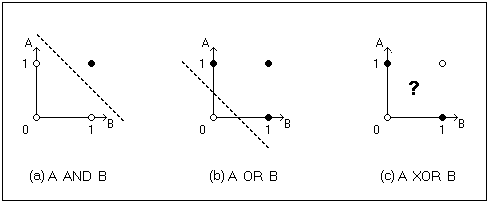
\includegraphics[scale = 0.8]{img.jpg}
    \caption{Linearly Separable and non-Linearly Separable Boolean Functions}
    \label{fig:my_label}
\end{figure}

\begin{itemize}
    \item The above table details the weights for some linearly separable Boolean functions of two inputs. 
    
    \item To represent XOR and XNOR functions, two neurons connected in sequence are required.
\end{itemize}

\subsection{Perceptron Training Rule}
\begin{itemize}
    \item The most common training algorithm for training of perceptrons is the \textbf{gradient descent} rule, where the weights are adjusted in an iterative manner to prevent misclassification
    
    \item This method requires the definition of an \textbf{error function} (also known as a \textbf{cost function}) that denotes the error between the learned label and the actual label classified. One commonly used cost function is the mean squared error. 
    
    \begin{equation}
        E(\overrightarrow{w}) = \frac{1}{2} \sum_{i=1}^{n} (t_i - o_i)^2
    \end{equation}
    
    Where $t_i$ is the \textit{target label} for the $i^{th}$ example in the training data, and $o_i$ is the \textit{output label} outputted by the perceptron unit for the $i^{th}$ example in the training data. 
\end{itemize}

\begin{figure}[!h]
    \centering
    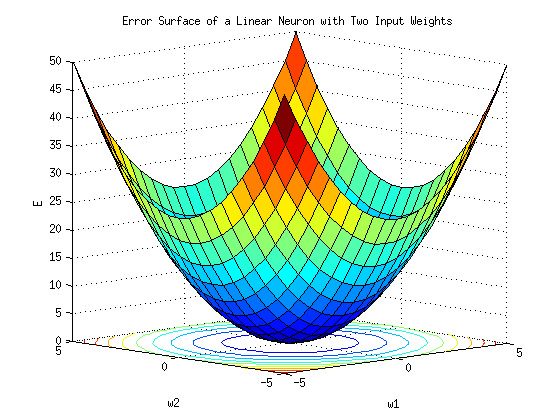
\includegraphics[scale = 0.6]{err.png}
    \caption{Error Surface for two weight perceptron}
    \label{fig:err}
\end{figure}

\begin{itemize}
    \item The gradient descent rule starts with an arbitrary vector of weights $(w_1, w_2, w_3, ..., w_n)$, and iteratively modifying this vector in small steps.
    
    \item The modification is done such that the vector moves towards the \textbf{global minimum} of the cost function. Hence the modification must be done in the direction of \textit{steepest descent} of the error surface.
    
    \item The direction of the steepest descent is given by the \textbf{negative of the gradient} of the error function. 
    
    \item The gradient of the error function is given as
    
    \begin{equation*}
        \nabla E = \left [ \frac{\partial E}{ \partial w_0}, \frac{\partial E}{ \partial w_1}, \frac{\partial E}{ \partial w_2}, ..., \frac{\partial E}{ \partial w_n}\right]
    \end{equation*}
    
    \item Therefore, the training rule for gradient descent is given as
    
    \begin{equation}
        w_i = w_i - \alpha \nabla E(w_i)
    \end{equation}
    
    \item This implies that each component $w_i$ of the weight vector $\overrightarrow{w}$ is modified in proportion to the partial derivative with respect to that component $\frac{\partial E}{\partial w_i}$
    
    \item The constant $\alpha$ is known as the \textit{learning rate}. It determines the speed at which the descent along the error surface takes place.
    
    \item It is important to find an optimal value for the hyperparameter $\alpha$ because too large a value may lead to overshooting the global minimum, but too small a value may lead to increased training time. 
    
    \item The gradient with respect to the kth weight $w_k$ can be calculated as 
    
    \begin{align*}
        \frac{\partial E}{\partial w_k} &=  \frac{\partial}{\partial w_k} \frac{1}{2} \sum_{i=1}^{n} (t_i - o_i)^2 \\
        &= \frac{1}{2} \sum_{i=1}^{n} \frac{\partial}{\partial w_k} (t_i - o_i)^2\\
        &= \frac{1}{2} \sum_{i=1}^{n} 2(t_i -o_i) \frac{\partial}{\partial w_k}(t_i -o_i)\\
        &= \frac{1}{2} \sum_{i=1}^{n} 2(t_i -o_i) \frac{\partial}{\partial w_k}(t_i - \overrightarrow{w}.\overrightarrow{x})\\
        &= \sum_{i=1}^{n} (t_i -o_i) (-x_{ik})\\
    \end{align*}
    
    \item $x_{ik}$ represents the value of the $k^{th}$ attribute of the $i^{th}$ training example. 
\end{itemize}

\subsection{Stochastic Gradient Descent (SGD)}
\begin{itemize}
    \item The gradient descent algorithm, as presented above, involves computing the cost function for \textbf{all the training examples at once} then and doing the weight update . 
    
    \item This is not only computationally expensive, but also does not guarantee that a global minimum will be reached in case the cost function has several local minima. 
    
    \item In \textit{stochastic gradient descent}, the weights are updated \textbf{for each training example at a time}. 
    
    \item The key differences between standard Gradient Descent and Stochastic Gradient Descent are:
    
    \begin{itemize}
        \item In standard gradient descent, the error is summed over all examples before updating weights, whereas in stochastic gradient descent weights are updated upon examining each training example.
        
        \item Stochastic Gradient Descent is capable of avoiding local minima, while Standard gradient descent is more susceptible to falling into a local minimum. 
        
        \item Summing over multiple examples in standard gradient descent requires more computation per weight update step than Stochastic Gradient Descent. 
        
        \item Because it uses the true gradient, standard gradient descent is often used with a larger step size per weight update (also known as the learning rate $\alpha$) than stochastic gradient descent.
    \end{itemize}
\end{itemize}

\section{Multi-Layer ANNs}
\begin{itemize}
    \item Multilayer networks in conjunction with non-linear \textbf{activation functions} are capable of learning a large variety of non-linear decision boundaries. 
    
    \item This make such networks more suited to a wider variety of tasks than single perceptron units. 
    
    \item The \textbf{backpropagation} algorithm is used to train multi-layer ANNs.
\end{itemize}

\subsection{Activation Functions}
\begin{itemize}
    \item Neurons that use he linear threshold function described in the above section is only capable of learning linear decision boundaries
    
    \item In order to learn more complex decision boundaries, a differentiable yet non-linear threshold is required. This non-linear threshold function is known as the activation function.
    
    \item Let the activation function be described as $\sigma(x)$. Then the computation of the neuron is described as
    
    \begin{align*}
        z = \sum_{i=0}^{n} w_i x_i \text{ where } x_0 = 1
    \end{align*}
    
    and the output $a$ of the neuron is written as
    
    \begin{align*}
        a = \sigma(z)
    \end{align*}
    
    \item Some popular activation functions are the \textbf{sigmoid}, the \textbf{tanh}, the \textbf{ReLU} and the \textbf{leaky ReLU} functions.
\end{itemize}

\subsubsection{Sigmoid Function}
\begin{itemize}
    \item The sigmoid function is given by
    \begin{equation*}
        \sigma(z) = \frac{1}{1+e^{-z}}
    \end{equation*}
    
    \item It's derivative, which is required for back propagation, is given by
    
    \begin{equation*}
        \sigma^{\prime} (z) = \sigma(z) ( 1- \sigma(z))
    \end{equation*}
    
    \item Advantages: Everywhere differentiable, easy to compute derivative, does not suffer from exploding gradients
    
    \item Disadvantages: Suffers from vanishing gradients (as $\sigma(z) \rightarrow 1 \text{ as } z \rightarrow \infty$, hence $\sigma(z)(1-\sigma(z)) \rightarrow 0$).
\end{itemize}

\subsubsection{tanh function}
\begin{itemize}
    \item The Hyperbolic tan function (tanh in short) is given by
    \begin{equation*}
        \sigma(z) = \frac{e^z - e^{-z}}{e^z + e^{-z}}
    \end{equation*}
    
    \item Its derivative is given as
    \begin{equation*}
        \sigma^{\prime}(z) = 1 - \sigma(z)^2
    \end{equation*}
    
    \item Advantages and disadvantages are similar to sigmoid function
\end{itemize}

\subsubsection{Rectified Linear Unit (ReLU)}
\begin{itemize}
    \item The ReLU function is given by
    
    \begin{equation*}
        \sigma(z) = \begin{cases}
            z \text{ if } z \ge 0 \\
            0 \text{ if } z < 0
        \end{cases}
    \end{equation*}
    
    \item Advantages: Does not suffer from vanishing gradients, easy to compute, better real-world performance than sigmoids
    
    \item Disadvantages: Suffers from exploding gradients as the value of activation is not constrained in the positive direction, suffers from Dying ReLU problem caused by too many negative activations (negative activations lead to 0 output, hence neuron does not learn anymore)
\end{itemize}

\subsubsection{Leaky Rectified Linear Unit (Leaky ReLU)}
\begin{itemize}
    \item The Leaky ReLU is given by
    
    \begin{equation*}
        \sigma(z) = \begin{cases}
            z \text{ if } z \ge 0 \\
            a z \text{ if } z < 0, \text{ where } 0 < a < 1
        \end{cases}
    \end{equation*}
\end{itemize}

\subsection{Backpropagation Algorithm}
\begin{itemize}
    \item Backpropagation is the most commonly used algorithm in multi-layer neural networks to minimize the cost function. 
    
    \item The derivation presented here is for Stochastic gradient descent, which considers the calculation for only one training example at a time. 
    
    \item Let $E_d$ be the error for one training example summed over all the units in the output layer of the multi-layer network.
    \begin{equation*}
        E_d = \sum_{k \in output\_units} (t_k - o_k)^2
    \end{equation*}
    
    \item The update rule can then be defined as:
    \begin{equation}
        \Delta w_{ji} = - \eta \frac{\partial E_d}{\partial w_{ji}}
    \end{equation}
    
    \item Nomenclature:
    \begin{enumerate}
        \item $x_{ji}$: The $i^{th}$ input to the $j^{th}$ unit. 
        
        \item $w_{ji}$: The weight associated with the $i^{th}$ input to the $j^{th}$ unit. 
        
        \item $net_j$: $\sum_{i} w_{ji}x_{ji}$, ie the weighted sum of inputs to the unit $j$
        
        \item $o_j$, $t_j$: Output and target of the $j^{th}$ unit. 
    \end{enumerate}
    
    \item For every training instance, the forward propagation step is done, and then the errors are propagated back (using the chain rule of differentiation) and then the weights are all modified. This is the stochastic version of back propagation. 
\end{itemize}

\subsubsection{Local Minima Avoidance in multilayer ANNs}
\begin{itemize}
    \item Using \textbf{stochastic} instead of batch gradient descent. As with SGD, the minimization of error happens over a different error function for each iteration, therefore on average, the likelihood that all the surfaces will descend into a local minima (and not a global one) is low. 
    
    \item Adding \textbf{momentum} to the gradient descent update rule. With the momentum term, the new update rule is given by
    \begin{equation*}
        \Delta w_{ji} (n) = \eta\text{ }\delta_j x_{ji} + \alpha \Delta w_{ji}(n-1)
    \end{equation*}
    here, $\Delta w_{ji}(n-1)$ is the update that occured to the weight $w_{ji}$ in the $n-1^{th}$ iteration. 
    
    \item Training multiple networks, each with \textbf{different initial weight values}. Either the best output can be selected (based on the validation data performance) or a weighted average of all the network's outputs can be used as the final prediction. 
\end{itemize}

\subsubsection{Preventing Overfitting in ANNs}
\begin{itemize}
    \item Make the model simpler (fewer layers, fewer units per layer)
    
    \item Regularization: A technique that places a penalty on the sum of the weights (L1) or the sum of squares of the weights (L2) by forcing that quantity to be minimized along with the loss function. The general formula for a loss function with L2 regularization is given as
    \begin{equation*}
        \mathbf{min}\text{ }L(y, \hat{y}) + \lambda \sum w_{ji}^2
    \end{equation*}
    
    \item Early Stopping is a technique wherein the model training is stopped (ie. the number of iterations is reduced) so as to combat overfitting on the train set. 
    
    \item Data Augmentation: Adding transformations of various types to the current data so as to obtain more data to train the model. 
\end{itemize}

\section{Support Vector Machines}
\begin{itemize}
    \item SVM is a supervised learning algorithm that can be used for both classification and regression tasks. 
    
    \item When classifying, the aim of an SVM is to construct the \textbf{maximum margin classifier}, ie. the classifier that maximises the distance between the positive and negative points. 
    
    \item Mathematically speaking, the SVM learns the equation of a linear decision hyperplane 
    \begin{equation*}
        y = \overrightarrow{w}x + b
    \end{equation*}
    Where w, b are parameters of the plane. 
    
    \item For convention, the values of $y$ for positive and negative examples are chosen as +1 and -1 respectively. 
    
\end{itemize}
\begin{figure}[!h]
    \centering
    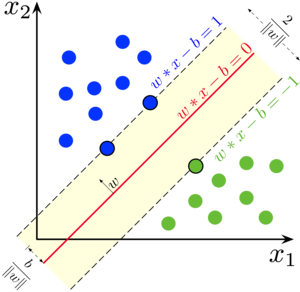
\includegraphics[scale=2]{svm.png}
    \caption{Support Vector Machine}
    \label{fig:my_label_1}
\end{figure}

\begin{itemize}
    \item For the positive and negative examples respectively, we have
    
    \begin{align*}
        \overrightarrow{w}.\overrightarrow{x} + b &\ge 1 \\
        \overrightarrow{w}.\overrightarrow{x} + b &\le -1
    \end{align*}
    
    \item Using the above definition of $y$, these can be combined into one equation
    \begin{equation}
        y.(\overrightarrow{w}.\overrightarrow{x} + b) -1 \ge 0
    \end{equation}
    
    \item For the points that lie \textit{on tha margins}, the $\ge$ becomes an equality sign. 
    
    \item Let $x_+$ and $x_-$ be a positive and negative example (these lie on the margins be definition). The width of the margin is
    \begin{equation*}
        d_m = \frac{\overrightarrow{w}}{||\overrightarrow{w}||} (\overrightarrow{x_+} - \overrightarrow{x_-})\\
    \end{equation*}
    
    substituting from equation (7), we have
    \begin{align*}
        d_m &= \frac{1}{||\overrightarrow{w}||} (1 - b - (-1-b))\\
        d_m &= \frac{2}{||\overrightarrow{w}||}
    \end{align*}
    
    \item Minimizing the quantity $\frac{2}{||\overrightarrow{w}||}$ can be shown to be equivalent to maximizing the quantity $\frac{1}{2}  ||\overrightarrow{w}||^2$ subject to the constraint in equation (7). 
\end{itemize}
\subsection{Constrained Optimization using Lagrangians}
\begin{itemize}
    \item First, the Lagrangian $\mathbb{L}$ is constructed as
    
    \begin{equation}
        \mathbb{L} = \frac{1}{2}  ||\overrightarrow{w}||^2 - \sum_{i=1}^{m} \alpha_i [y.(\overrightarrow{w}.\overrightarrow{x} + b) -1]
    \end{equation}
    
    \item Where $\alpha_i$ is the \textbf{Lagrange Multiplier} for the ith training example. The summation is over the training examples. 
    
    \item We compute the partial derivatives of the Lagrangian with respect to the parameters that are to be learnt, and set all the partial derivatives to 0. 
    \begin{align*}
        \frac{\partial \mathbb{L}}{\partial w} &= \overrightarrow{w} - \sum_{i=1}^{m} \alpha_i \overrightarrow{x_i} y_i = 0\\
        \overrightarrow{w} &= \sum_{i=1}^{m} \alpha_i \overrightarrow{x_i} y_i
    \end{align*}
    and
    \begin{align*}
        \frac{\partial \mathbb{L}}{\partial b} = - \sum_{i=1}^{m} \alpha_i y_i &= 0\\
        \sum_{i=1}^{m} \alpha_i y_i &= 0
    \end{align*}
    
    \item By substituting these values back in the Lagrangian, we obtain the \textbf{Lagrangian Dual} $\mathbb{L}_d$
    \begin{equation*}
        \mathbb{L}_d  =  \frac{1}{2} \sum_{i=1}^{m} \alpha_i \overrightarrow{x_i} y_i \sum_{j=1}^{m} \alpha_j \overrightarrow{x_j} y_j - \left [ \sum_{i=1}^{m} \alpha_i \overrightarrow{x_i} y_i  \sum_{j=1}^{m} \alpha_j \overrightarrow{x_j} y_j - \sum_{i=1}^{m} \alpha_i \right]
    \end{equation*}
    
    which gives:
    \begin{equation}
        \mathbb{L}_d = \sum_{i=1}^{m} \alpha_i -  \frac{1}{2} \sum_{i=1, j=1}^{m, m} \alpha_i  y_i \alpha_j  y_j (\overrightarrow{x_i} . \overrightarrow{x_j})
    \end{equation}
    
    \item The problem now reduces to
    \begin{align*} 
        \mathbf{max}\text{ }\mathbb{L}_d & \\
        \text{st. } \sum_{i=1}^{m} \alpha_i y_i &= 0 \\
        C > \alpha_i &> 0\text{ }\forall\text{ }i
    \end{align*}
    
    \item The constraint $C$ on the value of $\alpha$ is called the \textbf{slack} condition, which ensures that $\alpha$ does not go to infinity in case of a misclassification. 
    
    \item The solution to the Lagrangian dual is obtained by solving $\frac{\partial \mathbb{L}_d}{\partial \alpha} = 0$ for the value of $\alpha$. This value of $\alpha$ is subsituted above to get the value of $w$ and $b$ for the max margin classifier. 
    
    \item The final solution needs to satisfy the \textbf{Karush-Kuhn-Tucker} conditions (as the constraint involves an inequality). These are:
    \begin{enumerate}
        \item \textbf{Stationary Condition}:
            \begin{align*}
                \frac{\partial \mathbb{L}}{\partial w} &= 0\\
                \frac{\partial \mathbb{L}}{\partial b} &= 0
            \end{align*}
            
        \item \textbf{Primal Feasibility}: 
        \begin{equation*}
            y.(\overrightarrow{w}.\overrightarrow{x} + b) -1 \ge 0\text{ }\forall\text{ }i
        \end{equation*}
        
        \item \textbf{Dual Feasibility}:
        \begin{equation*}
            \alpha_i\ge0\text{ }\forall\text{ }i
        \end{equation*}
        
        \item \textbf{Complementary Slackness}:
        \begin{equation*}
            \alpha_i [y.(\overrightarrow{w}.\overrightarrow{x} + b) -1] = 0
        \end{equation*}
    \end{enumerate}
    
    \item From the slackness condition, it can be derived that for all non-support vectors, the value of $\alpha_i$ is 0. This means that the majority of $\alpha_i$ are 0, leading to less memory needed to store them. 
\end{itemize}
\end{document}

